% TODO make sure quoted values are accurate (i.e. look em up)
\section{Results}
This section is split into two parts, the first looking at the results
of our cloud coverage analysis and the second looking into the NDVI
analysis.
\subsection{Cloud Coverage}
\subsubsection{Rainfall}
Figure \ref{fig:cf_rf} shows the monthly averages of cloud fraction over the
period $2008-2017$ and rainfall over the period $1991-2015$ for South Africa
(Figure \ref{fig:cf_rf_south}) and East Africa (Figure
\ref{fig:cf_rf_east}). For both cloud fraction and rainfall, a sinusoidal curve
with a period of $T=12$ months has been fitted to better highlight the seasonal
dependencies. From Figure \ref{fig:cf_rf_south} we see that South Africa has the
largest values of cloud fraction and rainfall at the beginning and end of the
year (local summer), with cloud coverage of ${\sim}0.2-0.3$ and rainfall of
${\sim}70$ mm. During the middle of the year (local winter), cloud coverage falls
below $0.1$ and rainfall drops to ${\sim}20$ mm. Now looking at Figure
\ref{fig:cf_rf_east} we see the opposite trend for East Africa. Cloud coverage
and rainfall are at there smallest values at the beginning and end of the year
(local winter), at ${\sim}0.4$ and ${\sim}21$ mm respectively. As we head toward the
middle of the year (local summer), cloud coverage and rainfall peak at
${\sim}0.3$ and $24$ mm respectively.
\begin{figure}
  \begin{subfigure}{\linewidth}
    \centering
    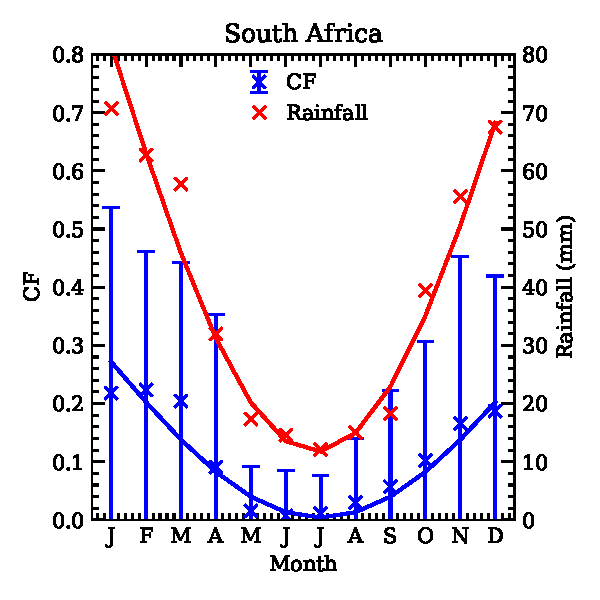
\includegraphics[width=0.85\linewidth]{figures/cf_rainfall_capetown}
    \caption{South Africa}
    \label{fig:cf_rf_south}
  \end{subfigure}
  \begin{subfigure}{\linewidth}
    \centering
    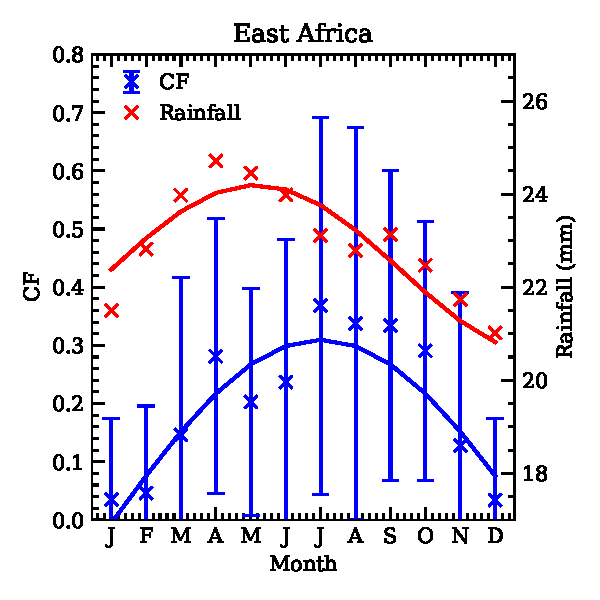
\includegraphics[width=0.85\linewidth]{figures/cf_rainfall_eastafrica}
    \caption{East Africa}
    \label{fig:cf_rf_east}
  \end{subfigure}
  \caption{Monthly averages of cloud fraction over the period
    $2008-2017$ (blue), with associated uncertainties and a fitted
    sinusoidal curve with fixed period $T=12$ months. Also shown are
    monthly averages of rainfall data over the period $1991-2015$
    (red) for South Africa (top) and Ethiopia (bottom) and fits of
    sinusoidal curves with period again fixed at $T=12$ months.}
  \label{fig:cf_rf}
\end{figure}

\subsubsection{SSTA}
Figure \ref{fig:cf_temporal} shows the dynamics of cloud coverage
anomalies between March 2008 and July 2017 for South Africa (Figure
\ref{fig:cf_t_south}) and East Africa (Figure \ref{fig:cf_t_east}) and
associated uncertainty, indicated by the shaded region. Also plotted
are the ONI and the relevant Indian Ocean SSTAs -- SWIO
for South Africa and WTIO for East Africa.
\begin{figure*}
  \centering
  \begin{subfigure}{\textwidth}
    \centering
    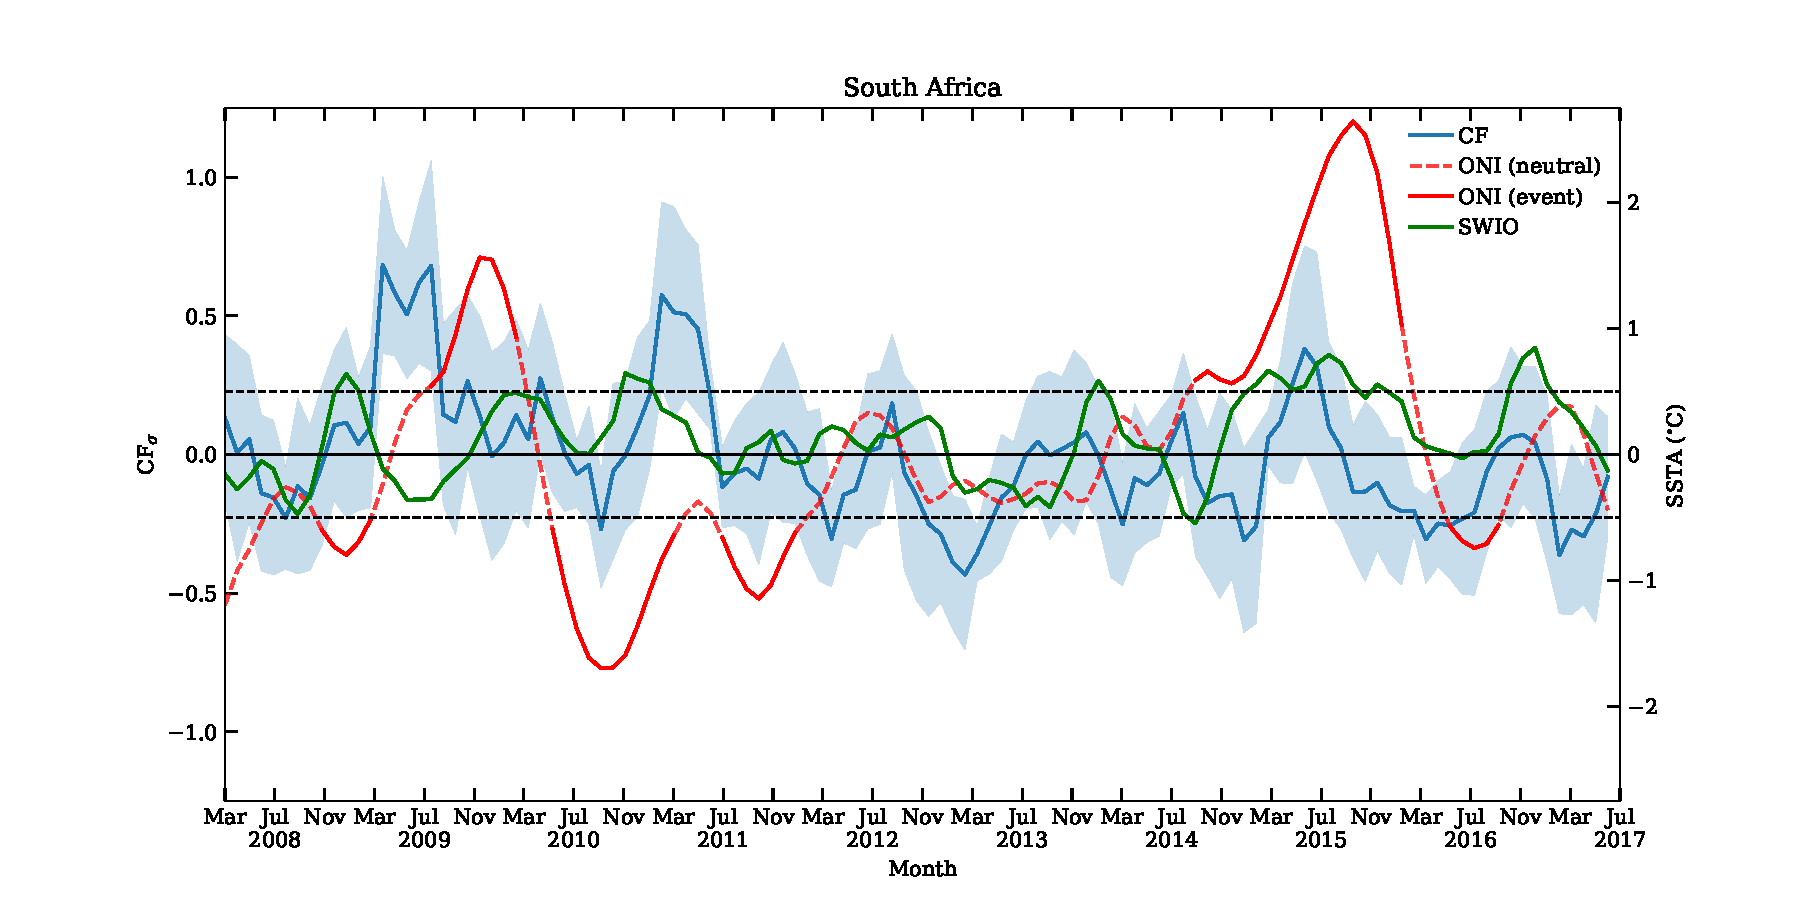
\includegraphics[width=\textwidth]{figures/cf_oni_io_capetown_5window_median}
    \caption{South Africa}
    \label{fig:cf_t_south}
  \end{subfigure}
  \begin{subfigure}{\textwidth}
    \centering
    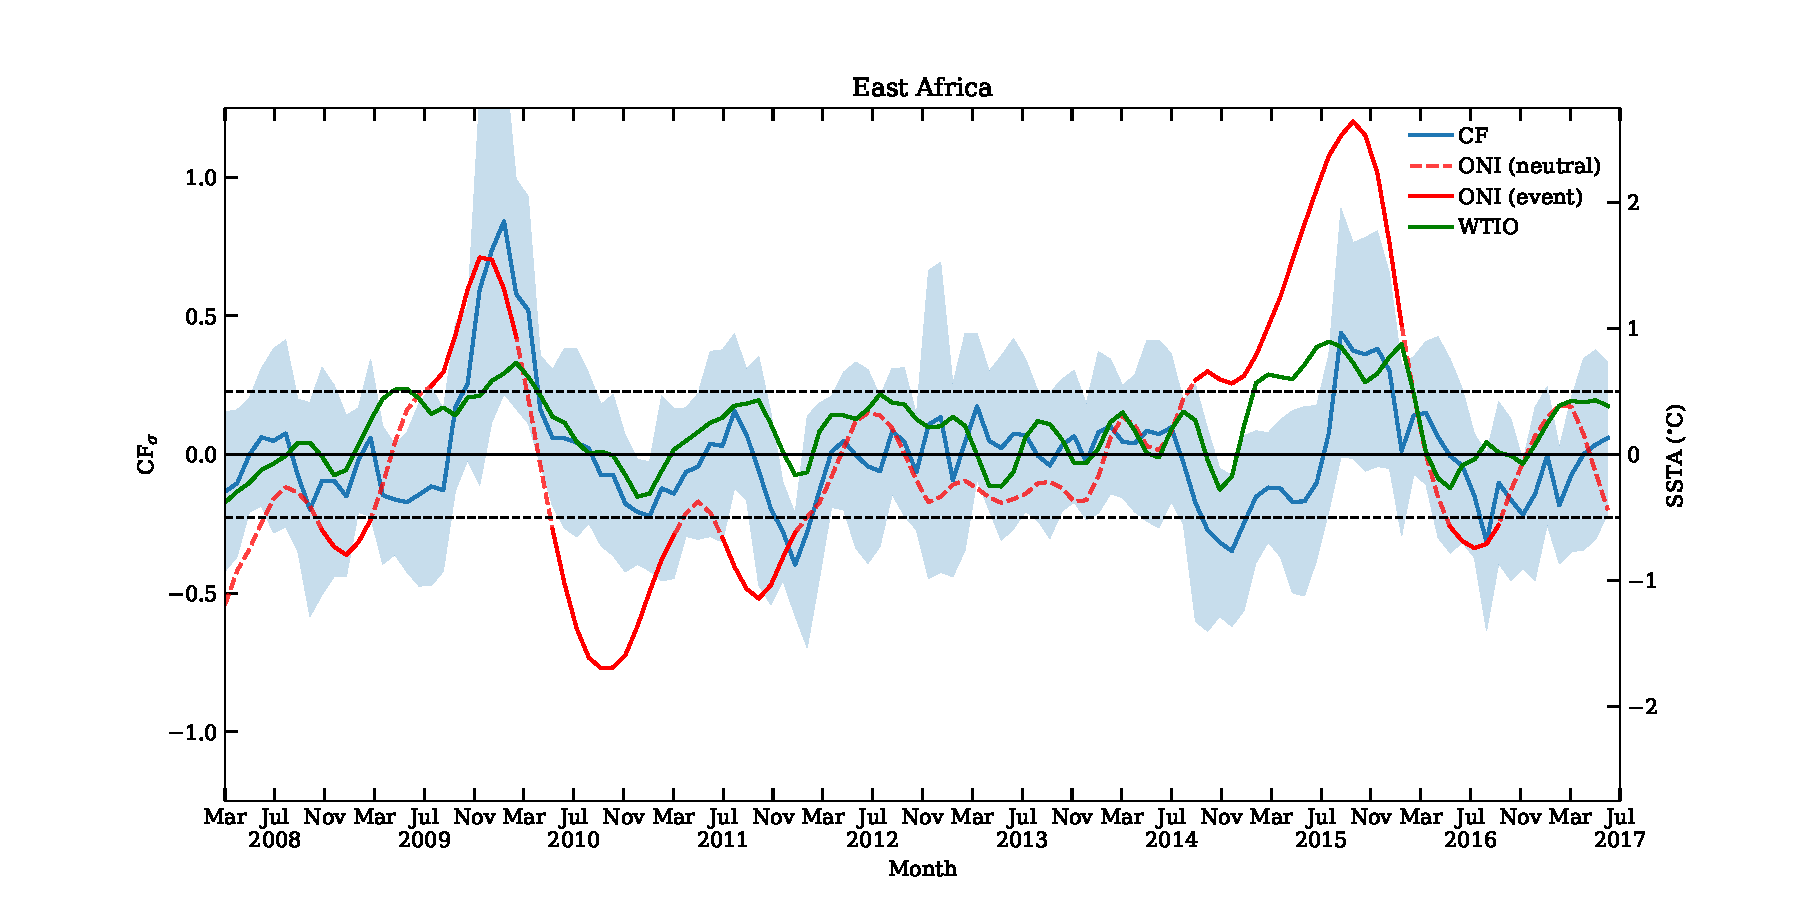
\includegraphics[width=\textwidth]{figures/cf_oni_io_eastafrica_5window_median}
    \caption{East Africa}
    \label{fig:cf_t_east}
    \end{subfigure}
  \caption{Time series of cloud fraction anomalies (blue) and
    uncertainty (shaded blue) from March 2008 to July 2017. Overlaid
    are the ONI (solid red line during ENSO events, dashed red line
    otherwise) and Indian Ocean SST anomalies (SSTA) for the relevant
    part of the Indian Ocean (green, SWIO for South Africa and WTIO
    for East Africa). Dashed black lines indicate the $\pm0.5^{\circ}$C
    threshold for declaring ENSO events. Top panel: South
    Africa. Bottom panel: East Africa.}
  \label{fig:cf_temporal}
\end{figure*}

From Figure \ref{fig:cf_t_south} we can see that in many instances, the
cloud fraction anomalies for South Africa appear to be out of phase
with ENSO events, following a lag of ${\sim}3$ months. For example,
following the peak of the 2010 \nina{} event around November, we
observe a turnaround of cloud fraction anomalies from $-0.25$ to a
peak of $0.5$ by March 2011, which persists until around July of that
year. During the very strong \elnino{} event beginning in November
2014 we observe a positive cloud fraction anomaly, coinciding with
extended periods of positive SWIO SSTAs.

Looking at Figure \ref{fig:cf_t_east} we observe strong positive cloud
fraction anomalies following the peak of the \elnino{} events of
2009/2010 and 2014/2015, again with a lag of ${\sim}3$ months. However,
cloud fraction anomalies are suppressed during the growth of the
2014/2015 \elnino{} and appear to instead follow the negative WTIO
SSTAs. Negative cloud fraction anomalies are observed during the
2008/2009, 2010/2011, 2011/2012 and 2016 \nina{} events, exhibiting
the same time lag. During all of these periods, apart from the 2016
\nina{}, negative WTIO SSTAs are also present.

\subsection{Vegetation}
To maximise the benefits of using remote sensing, we have divided our
analysis of vegetation coverage into two parts: spatial response and
temporal dynamics.

\subsubsection{Spatial Response}
Figures \ref{fig:ndvi_sp_south} and \ref{fig:ndvi_sp_east} show the
spatial response of NDVI for South and East Africa respectively. The
images are divided up into two seasons, December-January-February
(DJF) and June-July-August (JJA) as these correspond to the extrema of
the seasonal modulation of cloud coverage (Figure \ref{fig:cf_rf}) and
so are the times when any anomalies will likely be most visible. Each
column is then further divided up into whether \elnino{}, \nina{} or
neutral conditions are present.

\begin{figure*}
  \centering
  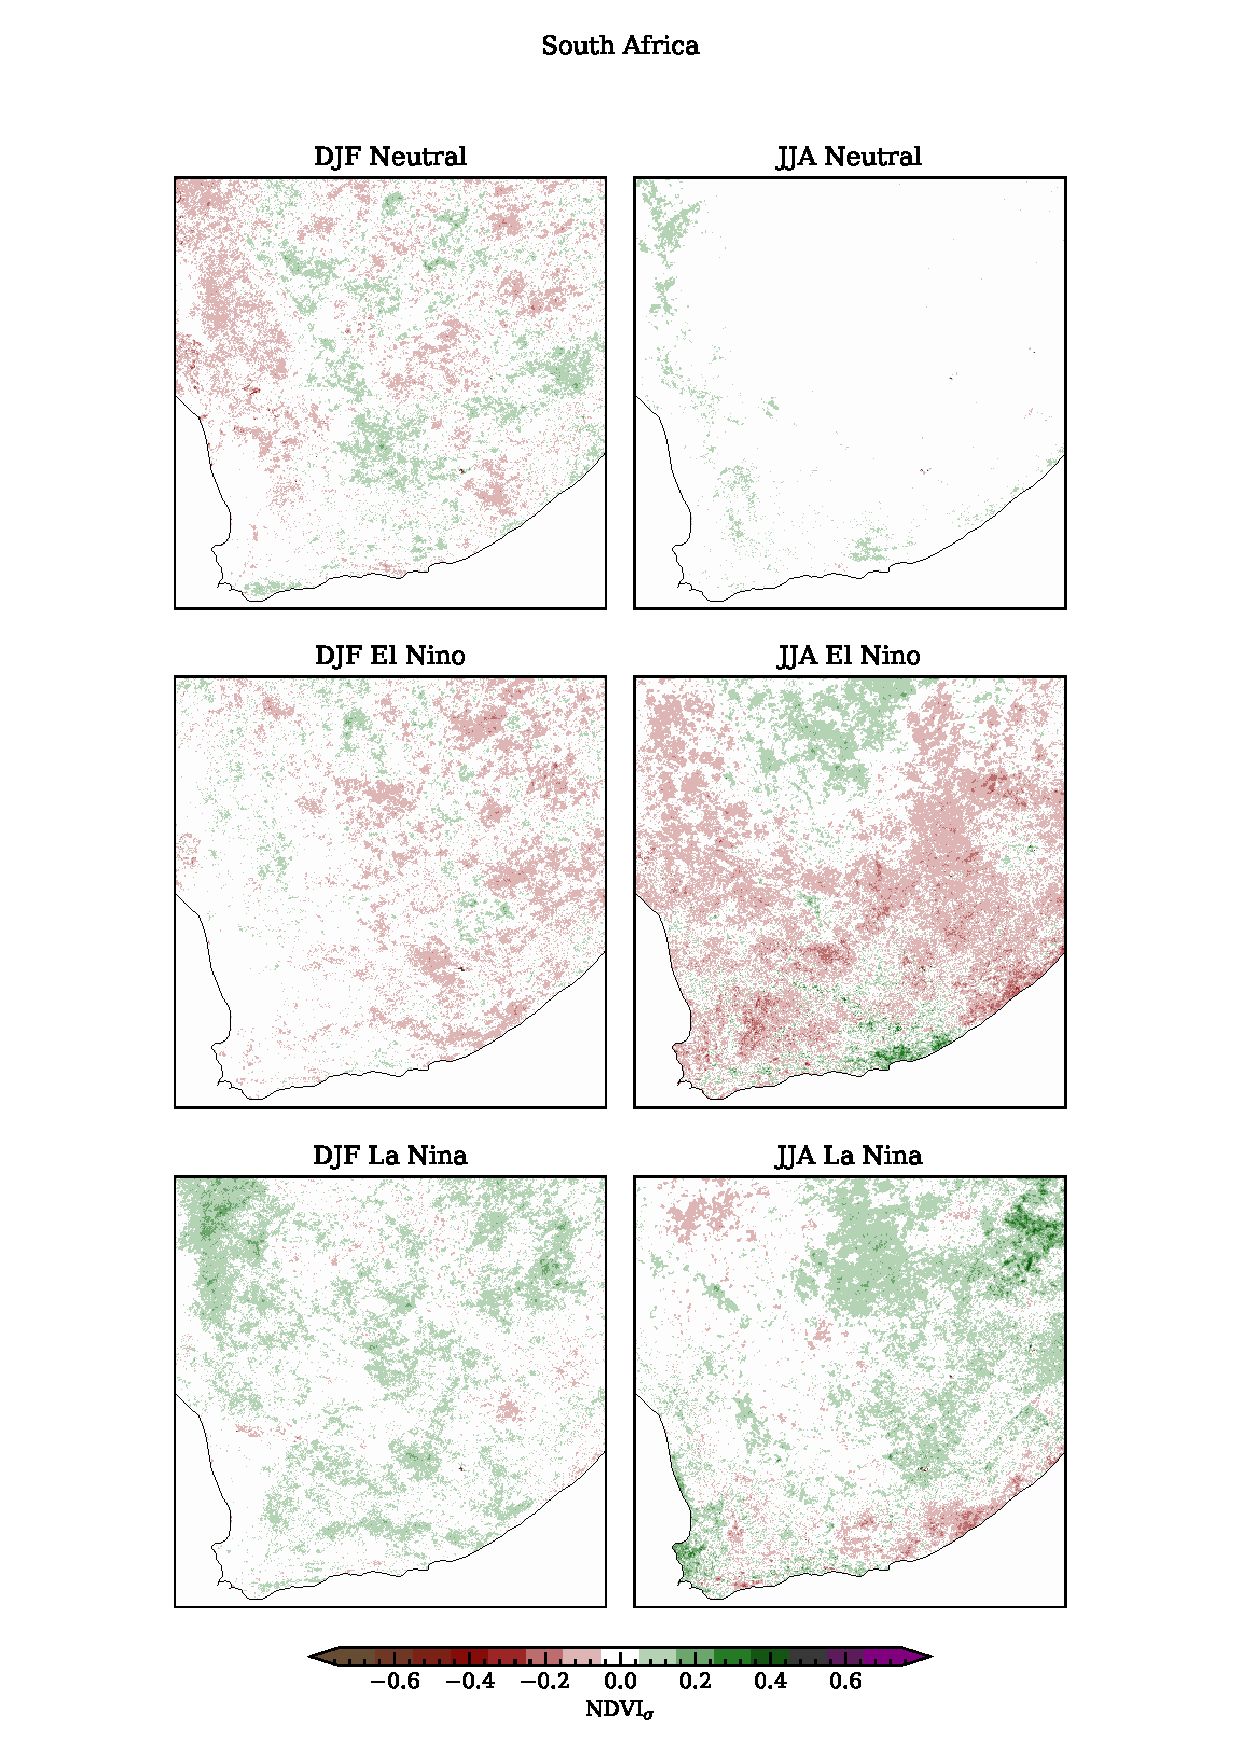
\includegraphics[height=0.9\textheight]{figures/ndvi_spatial_seasonal_anomalies_capetown}
  \caption{Spatial distribution of NDVI anomalies for South
    Africa. Three monthly means are taken for
    December-January-February (DJF) and June-July-August (JJA) and
    averaged again according to which phase of ENSO was present at the
    time.}
  \label{fig:ndvi_sp_south}
\end{figure*}

\begin{figure*}
  \centering
  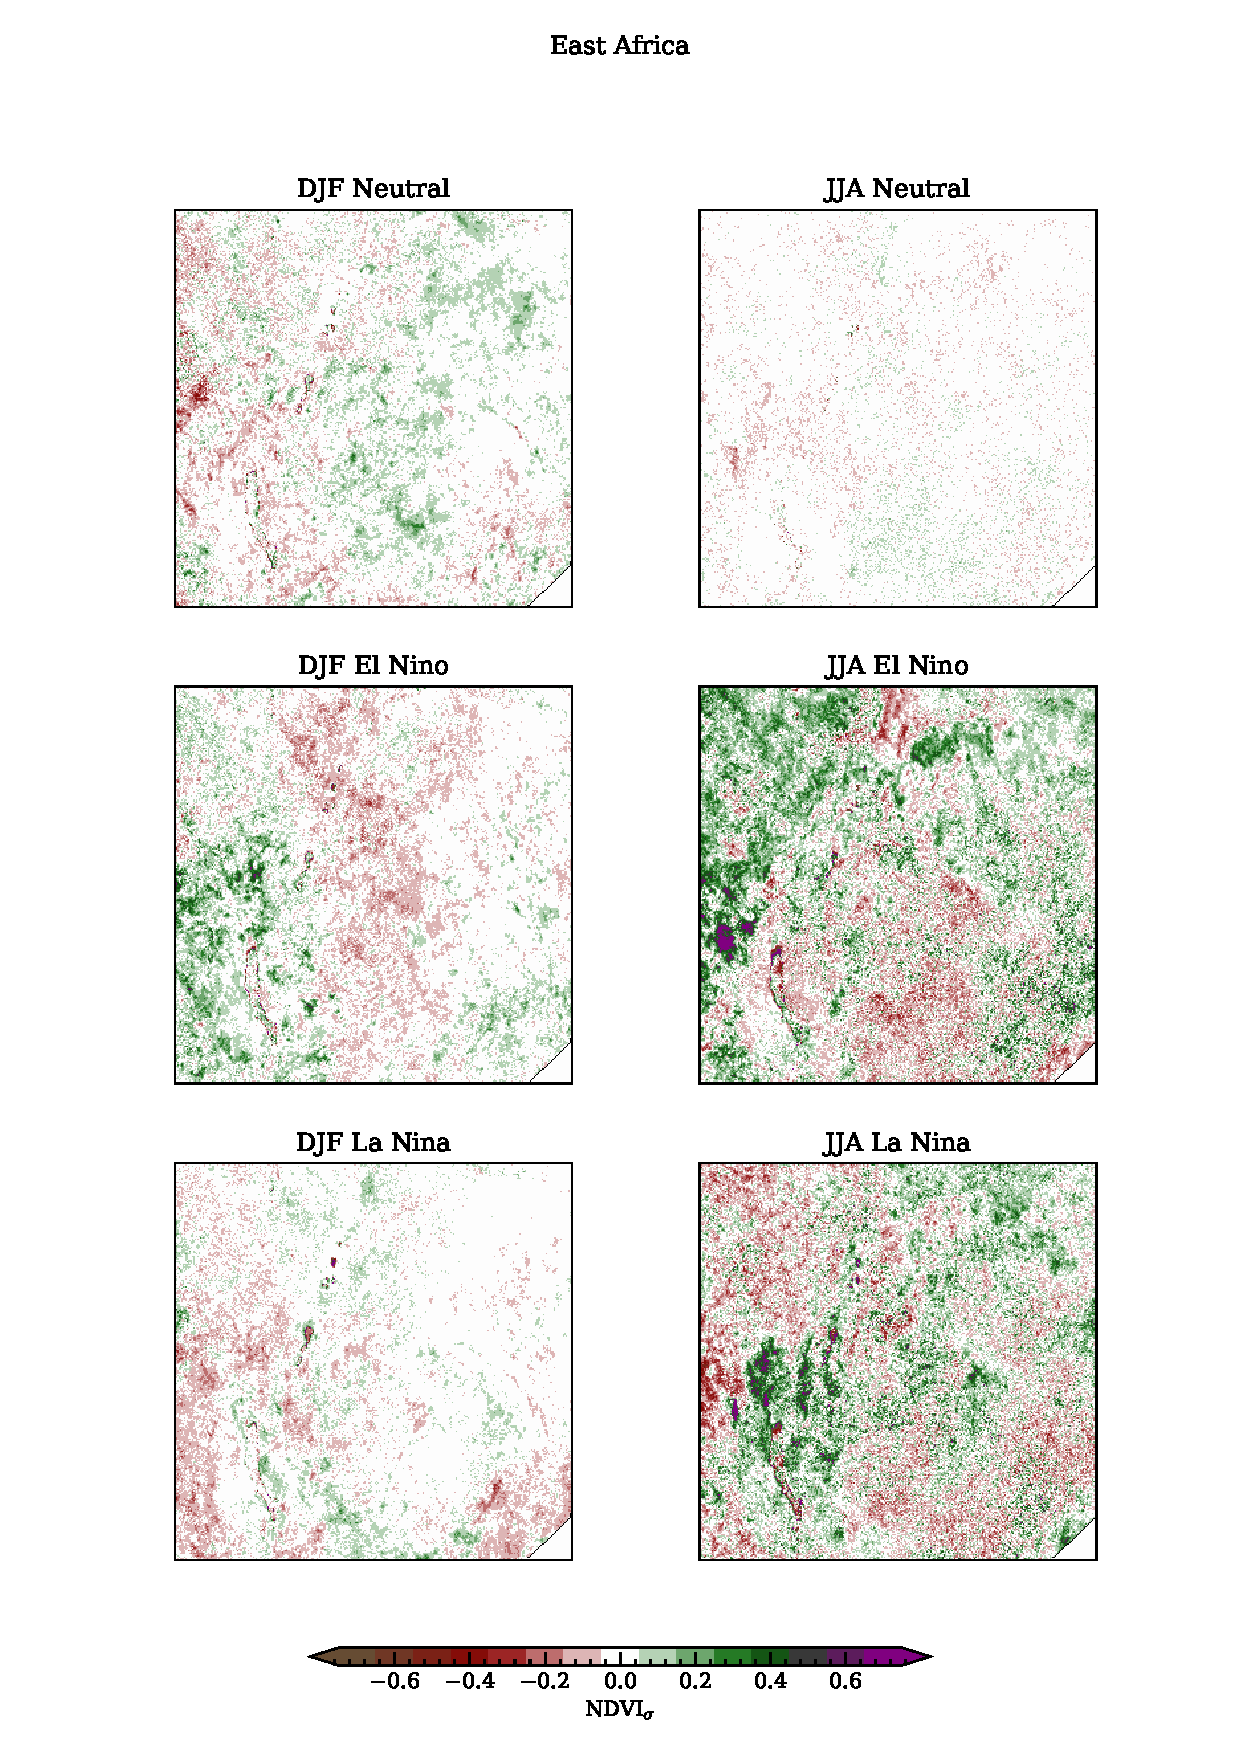
\includegraphics[height=0.9\textheight]{figures/ndvi_spatial_seasonal_anomalies_eastafrica}
  \caption{Spatial distribution of NDVI anomalies for East
    Africa. Three monthly means are taken for
    December-January-February (DJF) and June-July-August (JJA) and
    averaged again according to which phase of ENSO was present at the
    time.}
  \label{fig:ndvi_sp_east}
\end{figure*}

Looking first at South Africa, the top panels of Figure \ref{fig:ndvi_sp_south}
show that during neutral periods relatively small, evenly distributed anomalies
are present during DJF, while for JJA there are are mostly no anomalies, aside
from some small positive anomalies in the west. In the middle panels we can see
that during \elnino{} periods we observe a dearth of vegetation. These negative
anomalies are confined mostly to the east in DJF, while in JJA the anomalies
cover most of the region, with some positive anomalies appearing in the north
and along south-eastern coastal regions. Finally, the bottom panels show that
during \nina{} periods we observe an excess of vegetation, distributed fairly
evenly across the region for both periods. Some negative anomalies appear in the
north-west and along the south-eastern coast during JJA, in similar places to
the positive anomalies seen in JJA \elnino{}.

Moving now to East Africa, the top panels of Figure \ref{fig:ndvi_sp_east} show
a similar pattern to Figure \ref{fig:ndvi_sp_south}, namely that in neutral
periods anomalies are small and dispersed during DJF, although there does appear
to be a tendency for negative anomalies to appear in the south and positive
anomalies in the north. In JJA, anomalies are again essentially absent. For
\elnino{} periods, the middle left panel shows that, during DJF, there are
positive anomalies in the east, south-east and south-west and negative anomalies
in the centre, stretching from north to south. During JJA, the positive
anomalies in the east are very large and spatially concentrated, as are the
negative anomalies in the north; elsewhere positive and negative anomalies are
interspersed adjacently. During \nina{} events, positive anomalies concentrated
mostly in the south dominate during DJF. In JJA there is a mix of pockets of
high positive anomaly (e.g. the west and north-east) and positive anomaly
(e.g. far west, north west).

\subsubsection{Temporal Response}

\begin{figure*}
  \centering
  \begin{subfigure}{\textwidth}
    \centering
    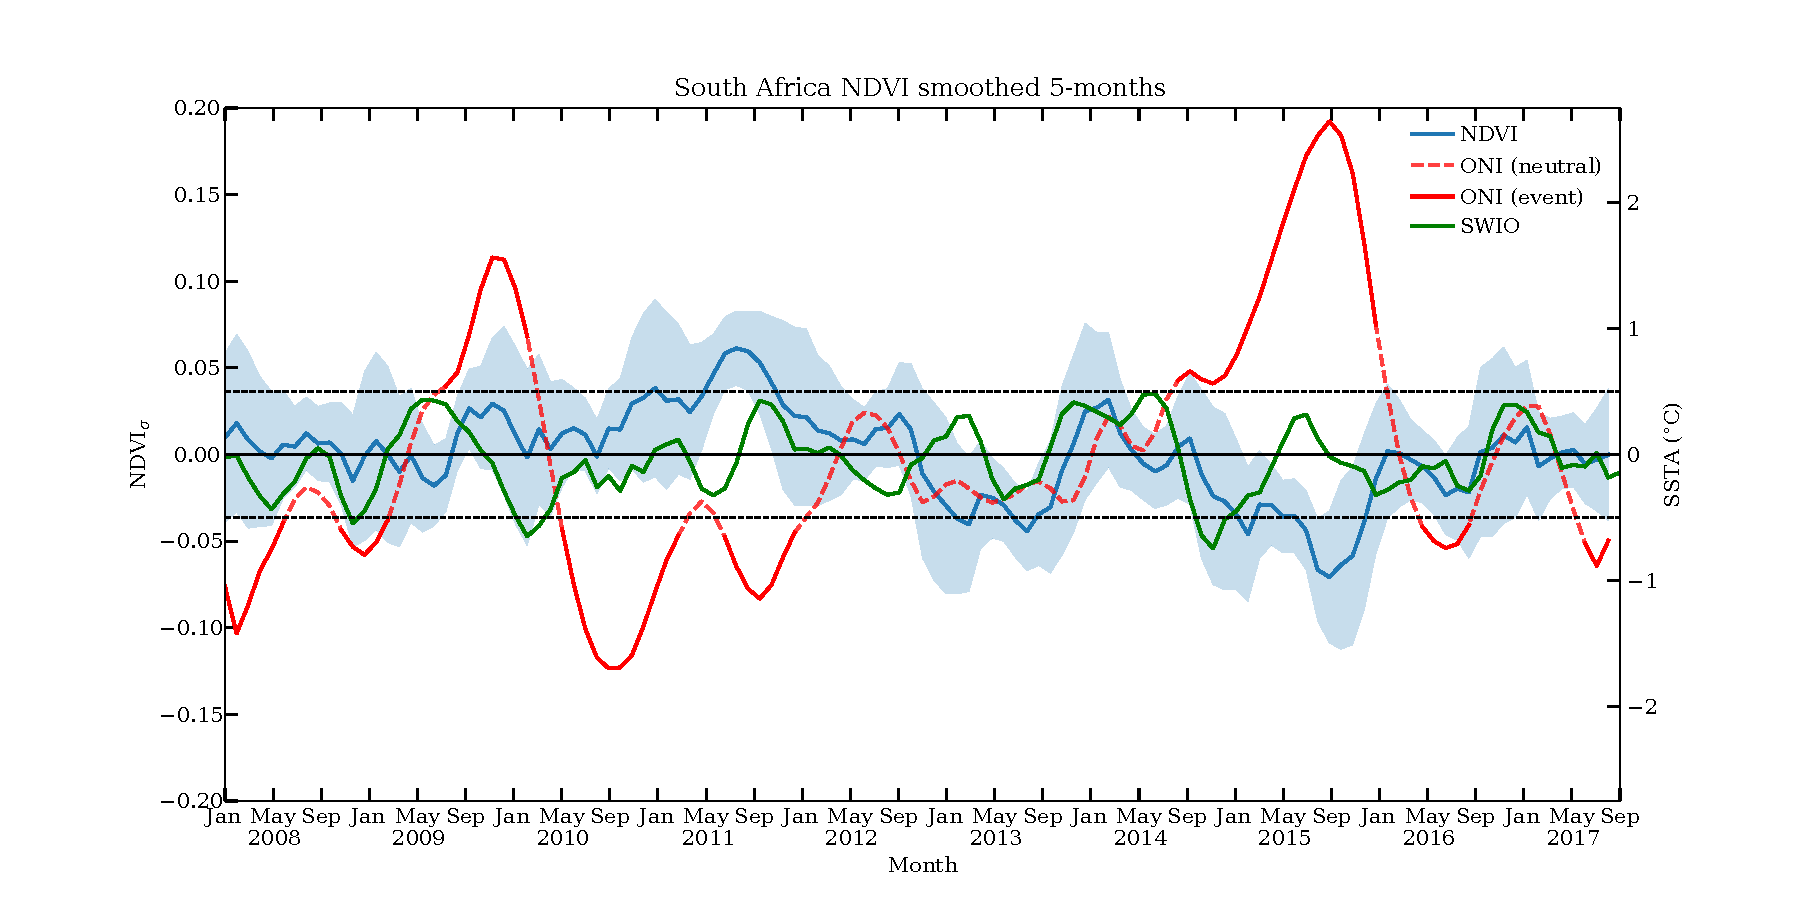
\includegraphics[width=\textwidth]{figures/ndvi_oni_io_capetown_smoothed_5.pdf}
    \caption{South Africa}
    \label{fig:ndvi_t_south}
  \end{subfigure}
  \begin{subfigure}{\textwidth}
    \centering
    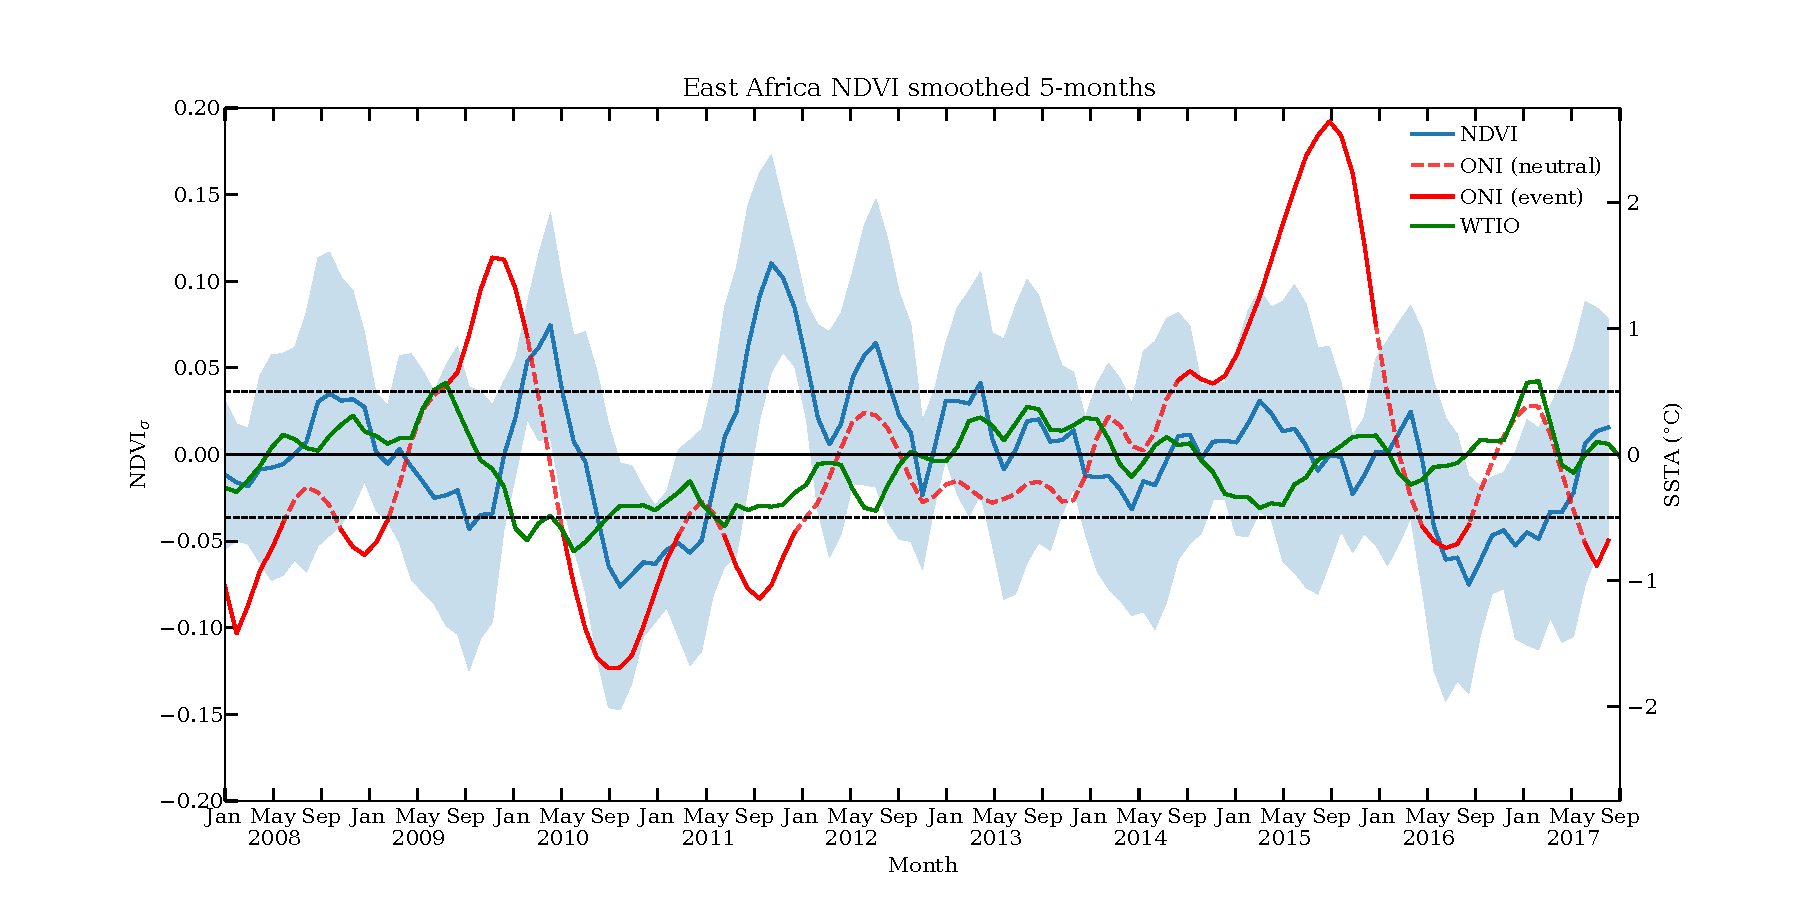
\includegraphics[width=\textwidth]{figures/ndvi_oni_io_eastafrica_smoothed_5.pdf}
    \caption{East Africa}
    \label{fig:ndvi_t_east}
    \end{subfigure}
  \caption{Time series of NDVI anomalies (blue) and uncertainty
    (shaded) from March 2008 to July 2017. Overlaid is ONI
    (red). Dashed black lines indicate the $\pm0.5^{\circ}$C threshold
    for declaring ENSO events. Top panel: South Africa. Bottom Panel:
    East Africa. Note worthy elements are for East Africa the period
    of January 2009 to May 2011, where a strong \elnino{} passes to a
    strong \nina{}; and for South Africa, the period May 2011 to May
    2016, where a similar reversal in ONI occurs. This is discussed
    further in \ref{sec:disc:ndvi}.}
  \label{fig:ndvi_temporal}
\end{figure*}

Figures \ref{fig:ndvi_t_south} and \ref{fig:ndvi_t_east} show the
temporal response of NDVI for South and East Africa respectively, over
the entirety of our ten-year dataset. Overlaid is the ONI that
is used to indicate when an \elnino{} or \nina{} event is occurring.

In both Figures \ref{fig:ndvi_t_south} and \ref{fig:ndvi_t_east} we
can make out the suggestion of correlation between ENSO and NDVI.

In South Africa, it appears that NDVI and ONI are
\emph{anti}-correlated, particularly during the \nina{} event in 2010
and the \elnino{} event in 2015. During the neutral ONI from 2012 to
2015, NDVI appears to follow the ONI trend closely. When the strong
\elnino{} appears in 2015, NDVI is similarly trending negative.

For East Africa, the relation appears to be in-phase, showing possible
correlation, with a strong \elnino{}-to-\nina{} reversal during 2009
being accompanied a slightly delayed peak-to-trough reversal in
NDVI. Following the 2010 \nina{}, a second \nina{} event occurs in
2011, this time however NDVI progresses out-of-phase climbing to its
maximal value. Between 2012 and 2015 there is a neutral ONI, with NDVI
in this region following a similar calm. The 2015 \elnino{} event
seems to stir NDVI out of its slumber, with a strong negative anomaly
in 2016.

%% Local Variables:
%% fill-column: 80
%% TeX-master: "report"
%% End:
